% !TeX root = 错题集模板.tex
% ============================================================
%  封面（错题集）：李思风（极简学术）—— 白底、居中标题、无装饰边框
%  参照《线性代数：原理与应用》（李思，清华大学）封面版式
%
%  可用字段（在主文件导言区 \newcommand 预定义即可覆盖）：
%    \notename      主标题（必填，主文件定义）
%    \noteauthor    作者（必填，主文件定义）
%    \notesubtitle  标题下方小字，默认 \today（日期/版本行）
%    \noteextra     底部单位/学院行，默认不显示
%
%  说明：中部线稿为可删装饰，整段 \begin{tikzpicture}...\end{tikzpicture}
%        删除后即为纯文字极简封面。
% ============================================================
\begin{titlepage}
	\thispagestyle{empty}
	\providecommand{\notesubtitle}{\today}
	\providecommand{\noteextra}{}
	\begin{center}
		\vspace*{4.7cm}

		% ---- 主标题 ----
		{\bfseries\songti\fontsize{24.8}{30}\selectfont \notename\par}

		\vspace{4.1cm}

		% ---- 日期 / 版本行 ----
		{\songti\fontsize{14.4}{18}\selectfont （\notesubtitle）\par}

		\vspace{3.4cm}

		% ---- 手绘风极简线稿：圆锥体积（可整段删除）----
		\begin{tikzpicture}[line width=0.8pt, line cap=round]
			% 底面椭圆与两条母线
			\draw (0,0) ellipse [x radius=1.3, y radius=0.36];
			\draw (-1.3,0) -- (0,2.3);
			\draw (1.3,0) -- (0,2.3);
			% 高（虚线）与底面半径
			\draw[dashed, line width=0.6pt] (0,0) -- (0,2.3);
			\draw[line width=0.6pt] (0,0) -- (1.3,0);
			\fill (0,0) circle (0.7pt);
			\node[font=\footnotesize] at (-0.38,1.15) {$h$};
			\node[font=\footnotesize] at (0.62,0.16) {$r$};
			% 体积公式
			\node[font=\small] at (3.1,1.15) {$V=\dfrac{1}{3}\pi r^{2}h$};
		\end{tikzpicture}

		\vspace{4.3cm}

		% ---- 作者（楷体）----
		{\kaishu\fontsize{24.8}{30}\selectfont \noteauthor\par}

		\vspace{1.8cm}

		% ---- 单位 / 学院（未定义则不显示）----
		{\songti\fontsize{20.7}{26}\selectfont \noteextra\par}

		\vspace*{1.6cm}
	\end{center}
\end{titlepage}
